\section{Mandelbrot}

\from{HIPS begin}
\subsection{HIPS}
The Mandelbrot~\cite{Mandelbrot-80} set are all complex numbers $c \in {\mathbb C}$ for which the sequence
\begin{equation}
	z_{i+1} = z_{i}^{2} + c, i\in {\mathbb N}
	\label{eq:mandelbrot}
\end{equation}
starting with $z_{0}=0$ does not escape to infinity.
If drawn as an image with each pixel representing a complex number, the boundary of the Mandelbrot set forms a fractal.
The calculation of such an image is a time-consuming task, because the sequence given by~(\ref{eq:mandelbrot}) has to be calculated for every pixel.
If this sequence does not cross a given threshold for a given number of steps, it is presumed that the sequence will converge.
The respective pixel is thus taken as a member of the Mandelbrot set, and it is painted black.
Other pixels outside are assigned a color that corresponds to the number of iterations of the sequence given by~(\ref{eq:mandelbrot}).
Computing a Mandelbrot fractal is easily parallelizable, as all pixels of the fractal can be computed simultaneously.

\subsubsection{Programming effort}
\label{sec:mandelbrot:implementation}

We created three similar parallel implementations for computing a Mandelbrot fractal using CUDA, OpenCL, and SkeCL.

CUDA and SkelCL require a single line of code for initialization in the host code, whereas OpenCL requires a lengthy creation and initialization of different data structures which take about 20 lines of code.

The host code differs significantly between all implementations.
In CUDA, the kernel is called like an ordinary function.
A proprietary syntax is used to specify the size of work-groups executing the kernel.
With OpenCL, several API functions are called to load and build the kernel, pass arguments to it and to launch it using a specified work-group size.
In SkelCL, the kernel passed to a newly created instance of a \texttt{Map} skeleton (see Section~\ref{sec:skeletons}).
A \texttt{Vector} of complex numbers, each of which is represented by a pixel of the Mandelbrot fractal, is passed to the \texttt{Map} skeleton upon execution.
Specifying the work-group size is mandatory in CUDA and OpenCL, whereas this is optional in SkelCL.
However, it is sometimes reasonable to also hand-optimize the work-group size in SkelCL, since it can have a considerable impact on performance.

\paragraph{Program size}
The OpenCL-based implementation has 118 lines of code (kernel: 28~lines, host program: 90~lines) and is thus more than twice as long as the CUDA and SkelCL versions with 49 lines (28, 21) and 57 lines (26, 31), respectively (see Figure~\ref{fig:mandelbrot_runtime}).
The length of the CUDA- and SkelCL-based implementations differs by only a few lines.

\paragraph{Kernel size}
The kernel function is similar in all implementations: it takes a pixel's position (i.e., a complex number) as input, performs the iterative calculation for this pixel, and returns the pixel's color.
However, while the input positions have to be given explicitly when using the \texttt{Map} skeleton in SkelCL, no positions are passed to the kernel in the CUDA- and OpenCL-based implementations.

\subsubsection{Performance experiments}
\label{sec:mandelbrot:runtime}

\begin{figure}[bp]
    \centering
    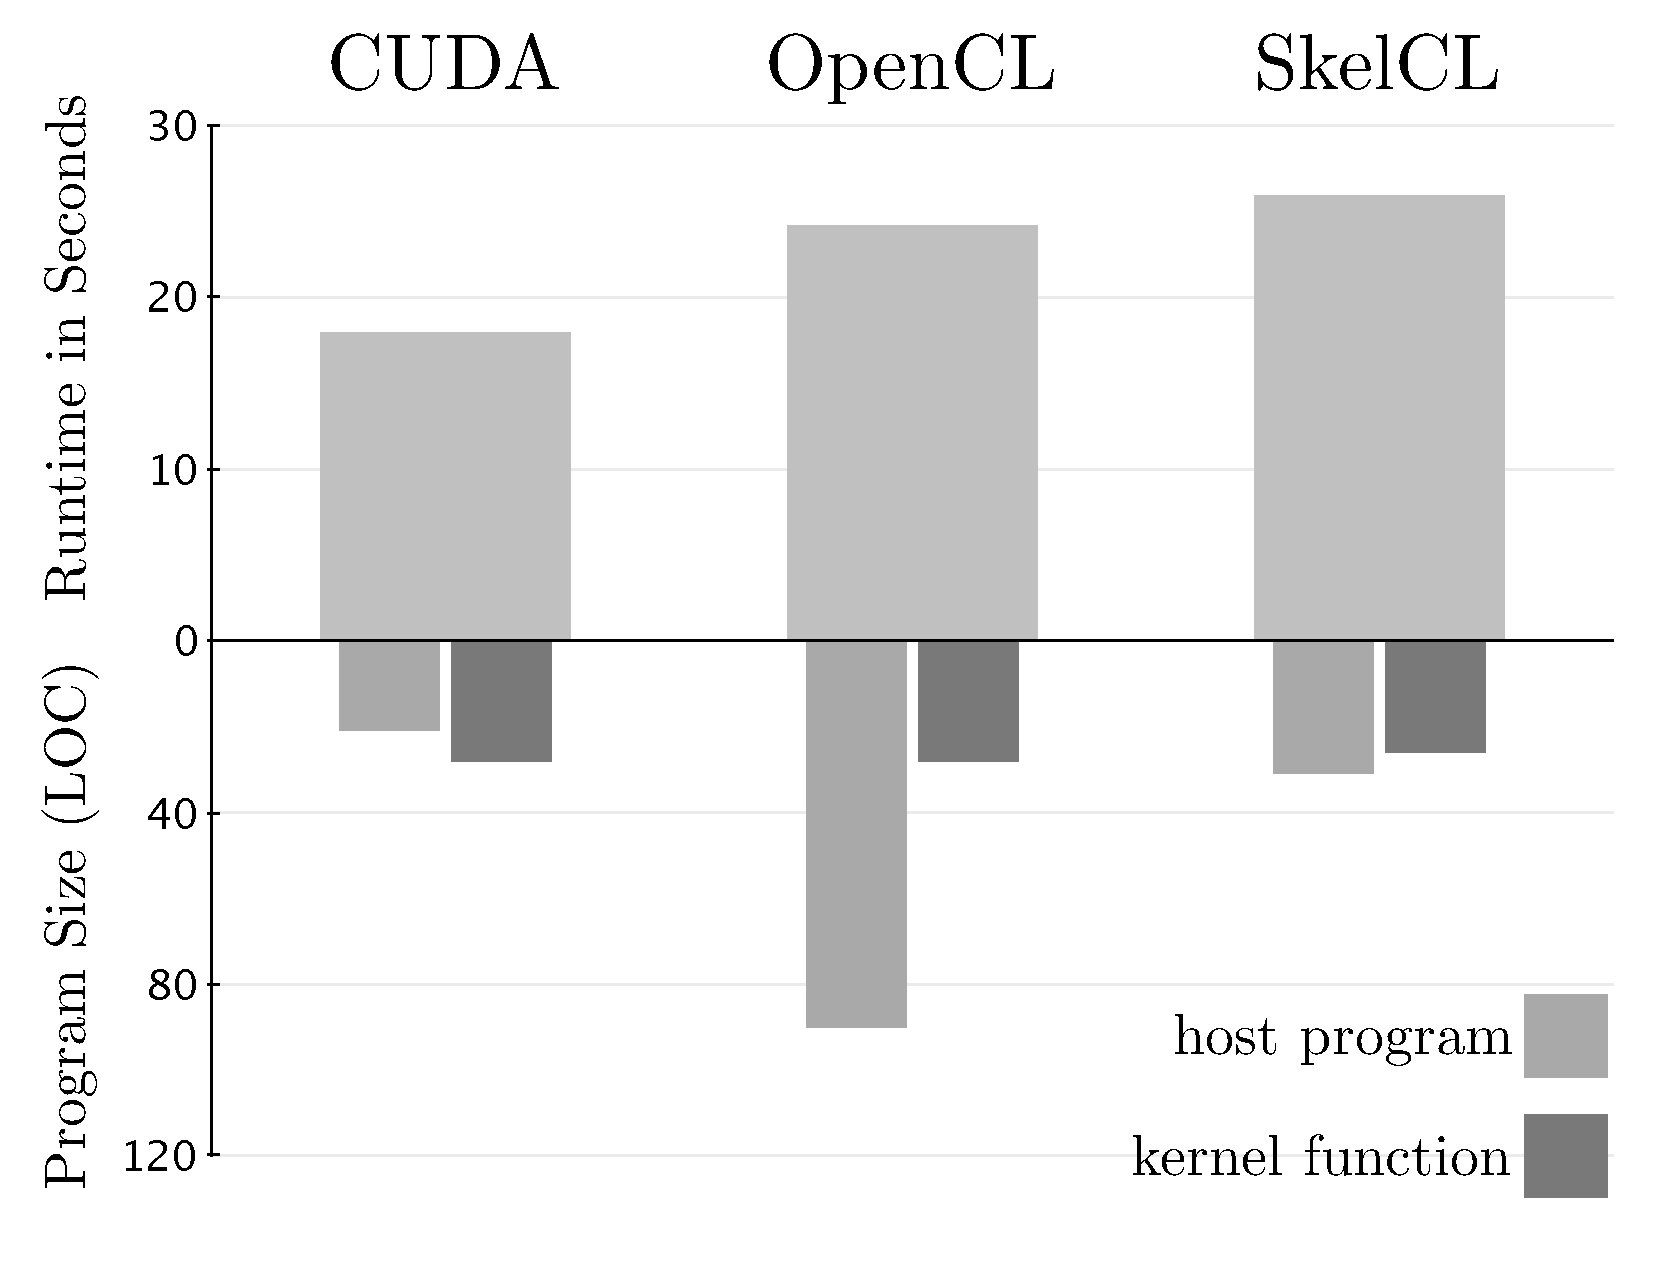
\includegraphics[width=0.42\textwidth]{HIPS/ChartMandelbrot}
    \caption{Runtime and program size of the Mandelbrot application.}
    \label{fig:mandelbrot_runtime}
\end{figure}%


We tested our implementations on a single GPU of our test system to compute a Mandelbrot fractal of size 4096$\times$3072 pixels.
In CUDA and OpenCL, work-groups of 16$\times$16 are used; SkelCL uses its default work-group size of~256.
The results are shown in Figure~\ref{fig:mandelbrot_runtime}.
As compared to the runtime of the SkelCL-based implementation (26 seconds), the implementation based on OpenCL (25 seconds) and CUDA (18 seconds) are faster by 4\% or 31\%, respectively.
Since SkelCL is built on top of OpenCL, the performance difference of SkelCL and OpenCL can be regarded as the overhead introduced by SkelCL\@.
Previous work~\cite{KoDYLCSMZ-10} also reported that CUDA was usually faster than OpenCL, which also explains the higher performance of the implementation based on CUDA.
The Mandelbrot application demonstrates that SkelCL introduces a tolerable overhead of less than 5\% as compared to OpenCL.
A clear benefit of this overhead is the reduced programming effort required by the SkelCL programm.
\from{HIPS end}


\from{PaCT begin}
\subsection{Application Study: Mandelbrot Set (PaCT)}
\label{sec:mandelbrot}

The Mandelbrot set calculation~\cite{Mandelbrot-80} is a time-consuming task which is often used as a benchmark. Computing a Mandelbrot fractal is easily parallelizable, as all pixels can be computed simultaneously.
As the criteria for programming effort we use the number of Lines of Code (LoC), the results are in Fig.~\ref{fig:mandelbrot_runtime}. 

We created three similar parallel implementations for computing a Mandelbrot fractal using CUDA, OpenCL, and SkeCL.

CUDA and SkelCL require a single line of code for initialization in the host code, whereas OpenCL requires a
\begin{figure}
    \centering
    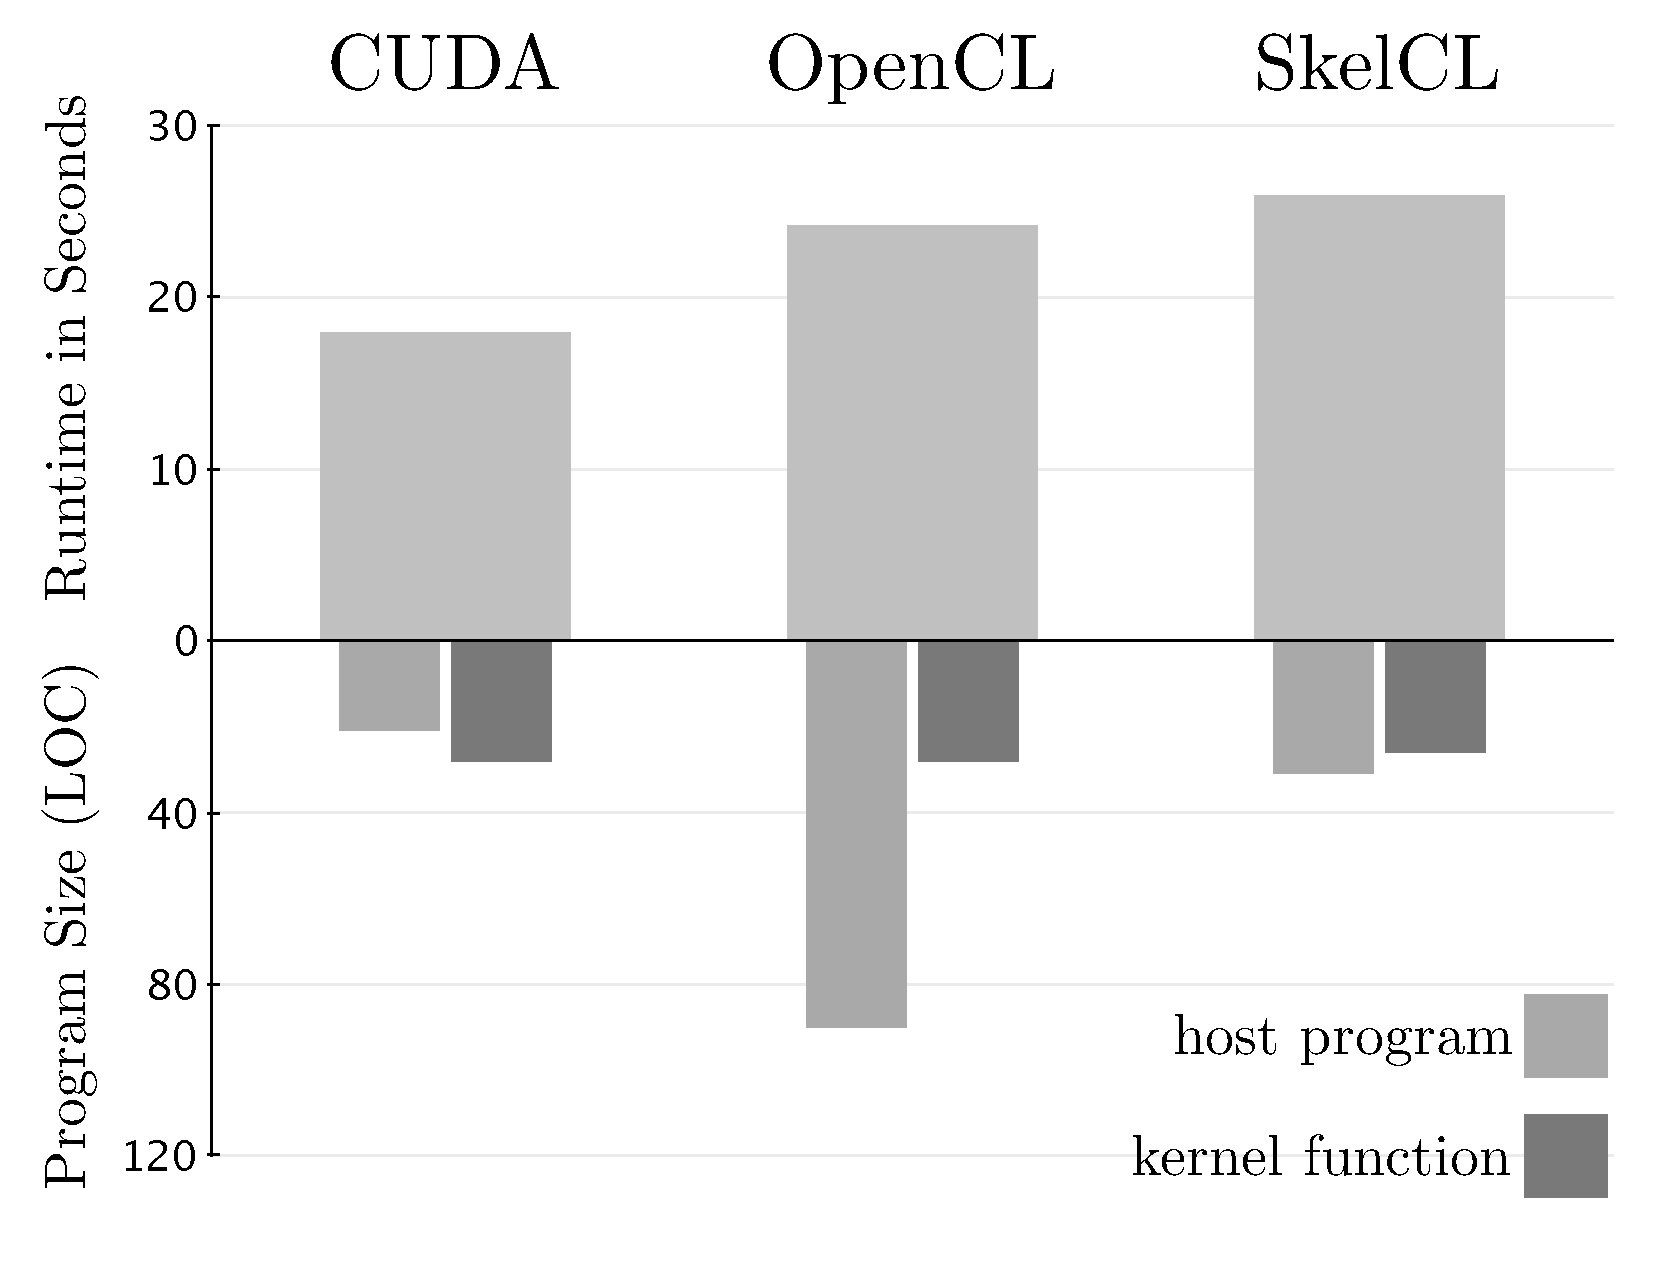
\includegraphics[width=0.6\textwidth]{PaCT/mandelbrotChartFinal.pdf}
    \caption{Runtime and program size of the Mandelbrot application.}
    \label{fig:mandelbrot_runtime}
\end{figure}%
lengthy creation and initialization of different data structures which take about 20 LoC.
The host CPU code differs significantly between all implementations.
In CUDA, the kernel is called like an ordinary function.
A proprietary syntax is used to specify the size of work-groups executing the kernel.
In OpenCL, several API functions are called to load and build the kernel, pass arguments to it and launch it using a specified work-group size.
In SkelCL, the kernel is passed to a newly created instance of the \texttt{Map} skeleton.
A \texttt{Vector} of complex numbers, each of which represents a pixel of the Mandelbrot fractal, is passed to the \texttt{Map} skeleton upon execution.
Specifying the work-group size is mandatory in CUDA and OpenCL, whereas this is optional in SkelCL.

The OpenCL-based implementation has in total 118 lines of code (kernel: 28~lines, host program: 90~lines) and is thus more than twice as long as the CUDA and SkelCL versions with 49 lines (28, 21) and 57 lines (26, 31), respectively (see Figure~\ref{fig:mandelbrot_runtime}).

We tested our implementations on a single GPU of our test system to compute a Mandelbrot fractal of size 4096$\times$3072 pixels.
In CUDA and OpenCL, work-groups of 16$\times$16 are used; SkelCL uses its default work-group size of~256.

As compared to the runtime of the SkelCL-based implementation (26 sec), the implementation based on OpenCL (25 sec) and CUDA (18 sec) are faster by 4\% or 31\%, respectively.
Since SkelCL is built on top of OpenCL, the performance difference of SkelCL and OpenCL can be regarded as the overhead introduced by SkelCL\@.
Previous work~\cite{KoDYLCSMZ-10} reported that CUDA was usually faster than OpenCL, which explains the higher performance of the implementation based on CUDA.
The Mandelbrot application demonstrates that SkelCL introduces a tolerable overhead of less than 5\% as compared to OpenCL.

\from{PaCT end}
